%%%%%%%%%%%%%%%%%%%%%%%%%%%%%%%%%%%%%%%%%%%%%%%%%%%%%%%%%%%%%%%%%%%%%%%%
%                                                                      %
%     File: Thesis_Background.tex                                      %
%     Tex Master: Thesis.tex                                           %
%                                                                      %
%     Author: Francisco Mendes                                         %
%     Last modified :  31 Jul 2020                                     %
%                                                                      %
%%%%%%%%%%%%%%%%%%%%%%%%%%%%%%%%%%%%%%%%%%%%%%%%%%%%%%%%%%%%%%%%%%%%%%%%

\chapter{Background}
\label{chapter:background}

This chapter provides an overview of modern \acrshort{gpu} architecture and the programming models that allow the extensive use of these devices in current applications, followed by an analysis of techniques to improve the energy efficiency of the same. 

The following sections present a bottom-up sequence of background and related work that supports this thesis—starting by the physical analysis of the digital circuits and the effects of V-F scaling and temperature on them. Continues by presenting the most common procedure to improve GPUs energy efficiency and finishes by exploring the techniques that will allow for further improvements to these devices. 

The relevance of the current work emerges from the reduced number of studies on the effects of decoupled voltage scaling on \acrshort{gpu}s, one of the objectives of this dissertation. The main reason is probably mainly due to lack of support for controlling these parameters on NVIDIA \acrshort{gpu}s (until recently, the dominant player on the market \cite{noauthor_jon_2018} \cite{mujtaba_amd_2019}) that is now allowed by the novel AMD software stack used on this work.






%%%%%%%%%%%%%%%%%%%%%%%%%%%%%%%%%%%%%%%%%%%%%%%%%%%%%%%%%%%%%%%%%%%%%%%%
\section{General Purpose Computing on GPUs}
\label{section:gpp_gpu}

A \acrshort{gpu} is a highly parallel programmable processor, that favours the execution of the same instruction on a set of data, belonging to the category of \textit{Single Instruction Multiple Threads} - \acrshort{simt} processors. When referring to \acrshort{gpu}s, it is still common to be talking about their graphics capabilities. However, more and more programs are taking advantage of their highly parallel architecture to accelerate general purpose applications, commonly referred to as \acrshort{gpgpu} - General Purpose Graphical Processing Unit.

The development and deployment of \acrshort{gpgpu} applications are only possible with the creation and adoption of standardized programming models and APIs that allow for hardware abstraction. This section provides a general overview of the \acrshort{gpu} architecture, followed by the presentation of the most common and used software tools available for \acrshort{gpgpu} programming.




\subsection{General Overview of a GPU Architecture}
The architecture of a modern GPU, figure~\ref{fig:Vega10arch}, can be roughly divided into computation and memory components. The computation part is usually composed of the vertex shader, the rendering engine, and the \acrshort{risc} processors. The vertex shader and rendering engine are included on the graphics pipeline and are not generally used on GPGPU applications. The RISC processors are responsible for the GPU programmable calculations and depending on the manufacturer, they are called streaming multiprocessors (\acrshort{sm}) in NVIDIA \acrshort{gpu}s \cite{nvidia_cuda_2008} or computing units (\acrshort{cu}) in AMD \acrshort{gpu}s \cite{amd_amd_2008}.  

\begin{figure}[htb]
  \begin{subfigmatrix}{2}
    \subfigure[Chip block diagram, example with 4 Compute Engines (RISC multi-processors), each with 16 NCU (Next Compute Units)]{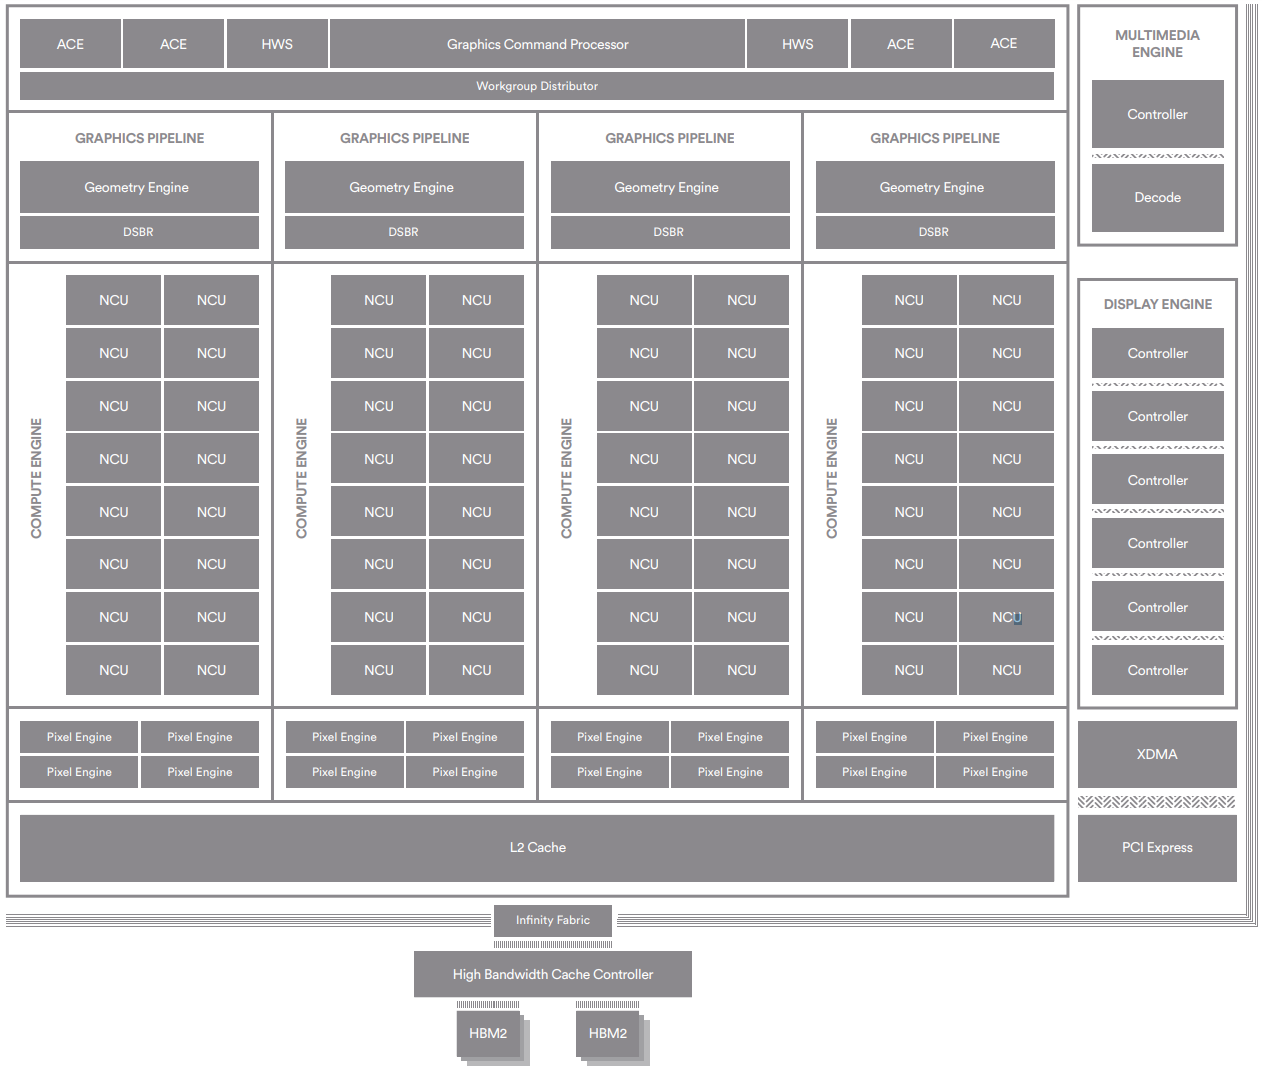
\includegraphics[width=0.7\linewidth]{Figures/Background/Vega10_microarchitecture.png}}
    \subfigure[NCU]{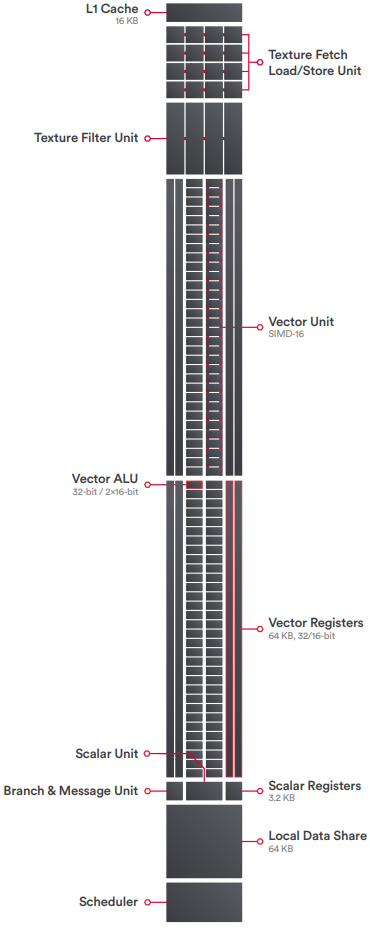
\includegraphics[width=0.24\linewidth]{Figures/Background/NCU.png}}
  \end{subfigmatrix}
  \caption{AMD's Graphics Core Next logical organization.}
  \label{fig:Vega10arch}
\end{figure}


One of the significant benefits of GPUs is, as said, the ability to concurrently execute multiple threads, for that, each SM or CU is made up of hundreds of execution units. However, to manipulate a such number of threads, it is necessary to have a significantly large and fast memory system, allowing to save the context of each thread and provide low-overhead context switching between the different sets of threads being executed. In that sense, modern GPUs architecture compresses a large register file on each \acrshort{sm}/\acrshort{cu}. For reference, in the AMD GNC architecture, each CU has 49,152 (32-bit) registers \cite{jing_energy-efficient_2013}.

In terms of memory, both the AMD and the NVIDIA GPUs present a 3 level hierarchy system: a global memory, accessible by all \acrshort{sm}/\acrshort{cu} (generally referred as video memory); a shared memory associated with each \acrshort{sm} or \acrshort{cu}, accessible by the threads running on that SM or CU; and a set of read-only caches for constants and textures, specific of each execution unit.

A GPU device from AMD will be used to conduct the experimental part of this dissertation. For that reason, the terminology used by AMD will be adopted. However, the presented work is independent of the hardware and terminology itself, and could equally be applied to NVIDIA \acrshort{gpu}s.

\subsection{GPU programming model}
The development of CUDA~\cite{nvidia_cuda_2017} (by NVIDIA) and OpenCL~\cite{noauthor_opencl_2013} (by Khronos Group) were the driving force to using \acrshort{gpu}s in general programming. CUDA and OpenCL are both parallel computing platforms and application programming interfaces (\acrshort{api}) that allow developers to create \acrshort{gpu}-accelerated applications, splitting the computations between the \acrshort{cpu} and \acrshort{gpu}. The first versions of these frameworks treated the \acrshort{gpu} as an accelerating slave device, providing a set of directives that allow the \acrshort{cpu} (master device) to transfer data, synchronize and control the \acrshort{gpu}.  Though, to take full advantage of the GPU architecture and create a true heterogeneous system, the \acrshort{cpu} and \acrshort{gpu} have to collaborate more efficiently. The creation of the Heterogeneous System Architecture (\acrshort{hsa}) \cite{hwu_heterogeneous_2015} framework acts on exactly improving this problem by acting as a low-level intermediary \acrshort{api} to provide improved coordination and communication for heterogeneous computing systems.  More recently, AMD introduced the Radeon Open Computing platform (\acrshort{roc}) \cite{noauthor_radeonopencompute/rocm_2019}. Just like CUDA and OpenCL, \acrshort{roc} provides a set of tools that allow developers to create heterogeneous applications. Being a newer software stack, already built on the notions and added benefits of \acrshort{hsa} runtime \acrshort{api}, ROC allows for the use of a wider set of programming frameworks like OpenCL, HC++, and HIP.



%%%%%%%%%%%%%%%%%%%%%%%%%%%%%%%%%%%%%%%%%%%%%%%%%%%%%%%%%%%%%%%%%%%%%%%%
\section{CMOS Circuit Characterization}
\label{section:CMOS}

For the last 40 years, CMOS (Complementary metal-oxide-semiconductor) is the most used technology in the creation of digital circuits and processors in general [REF]. 

There are two defined logic levels in digital circuits: logic level $0$ and $1$, each represented by an analog voltage range. The circuit requires a DC voltage value, $V_{DD}$, to operate and, the logic gates are excited through $V_{IN}$ and output, at $V_o$, the logic level correspondent to their logic function, Figure~\ref{fig:cmos}. As stated, the voltage range at the input of the logic gates is, following Figure~\ref{fig:cmos_noise_margin}, correctly interpreted if it falls inside a given range. Logic level $0$, from $GND$ ($0V$) to $V_{IL}$ and logic level $1$ from $V_{IH}$ to $V_{DD}$. In turn, the output is considered $0$ if it goes from $ GND $ ($0V$) to $V_{OL}$ and logic level $1$ from $V_{OH}$ to $V_{DD}$. The input and output logic levels' limits depend on the transistors' intrinsic characteristics, such as their dimensions and transconductance values. In addition to the transistors' characteristics, any digital circuit is also characterized by their frequency of operation.

\begin{figure}[htb]
    \centering
    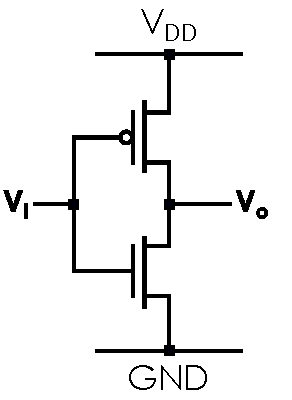
\includegraphics[width=30mm]{Figures/Background/cmos_inverter.pdf}
    \caption{CMOS inverter.}
    \label{fig:cmos}
\end{figure}

\begin{figure}[htb]
    \centering
    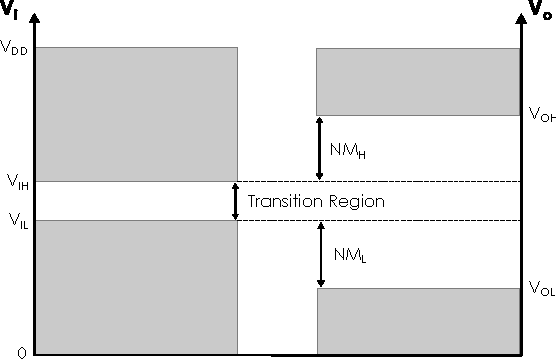
\includegraphics[width=85mm]{Figures/Background/voltage_margin.pdf}
    \caption{Noise margin definitions: $NM_L=V_{IL}-V_{OL}$ and $NM_H=V_{OH}-V_{IH}$.}
    \label{fig:cmos_noise_margin}
\end{figure}

This section provides an introduction to the effects of voltage and frequency scaling on the transistor and circuit level.

% Moore's law predicted the doubling of the transistors counts roughly every two years. The increase in the number of devices per chip directly translates to the observed performance increase over the last 60 years. However, in the last ten years, the industry is experiencing a slowdown. The shrinking of transistors is harder and harder and the amount of power created by today's chips is limits the transistor count (for the same node size). In this regard, it is indispensable that any digital circuit and, processors in particular, are develop taking into account the underlaying fabrication technology characteristics in order to find new ways of tackling this issues.

% The fundamental solution followed nowadays acts on varying the frequency and voltage values of the CMOS circuit accordingly to what is happening on the device. However, to take fully advantage of these parameters, it is critical to understand the impact of these variations on CMOS circuits.



\subsection{Propagation delay and Circuit critical path}

The propagation delay of a logic gate (e.g., inverter) corresponds to the difference in time (calculated at $50\%$ of input-output transition) between the output switching after the application of an input, as illustrated in Figure~\ref{fig:tp}. Considering both the transition low to high and high to low, the logic gate $tp$ corresponds to the average value of the two propagation delays, Equation~\ref{eq:tp_avg}.

\begin{figure}[htb]
    \centering
    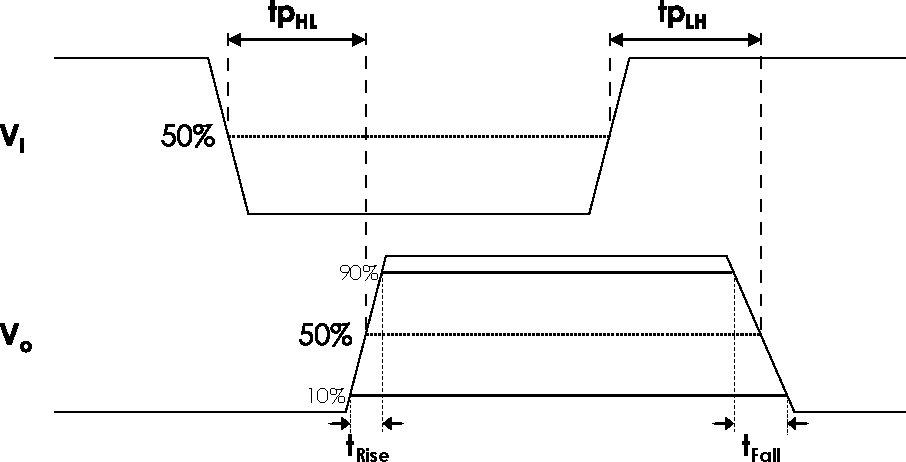
\includegraphics[width=80mm]{Figures/Background/propagation_delay.pdf}
    \caption{Logic gate propagation delay: $tp_{HL}$ - propagation delay high to low; $tp_{LH}$ - propagation delay low to high.}
    \label{fig:tp}
\end{figure}

\begin{equation}
    tp = tp_{avg} = \frac{tp_{HL}+tp_{LH}}{2}
    \label{eq:tp_avg}
\end{equation}

This metric is related to the time that the logic gate takes to switch its output logic level ($t_{Fall}$ for the high to low transition and $t_{Rise}$ for the low to high transition). This transition can be modeled as a first-order RC circuit, Figure~\ref{fig:rc_circuit}, with the transient response following Equation~\ref{eq:firtst_order}, where $\tau$ corresponds to the time constant. This time constant reflects the intrinsic characteristics of the transistors that make up the logic gate, being $\tau=RC$, where $R$ represents the average resistance of the transistor when it is turned 'ON' and $C$ the output capacitance that the logic gate is driving.


\begin{figure}[htb]
    \centering
    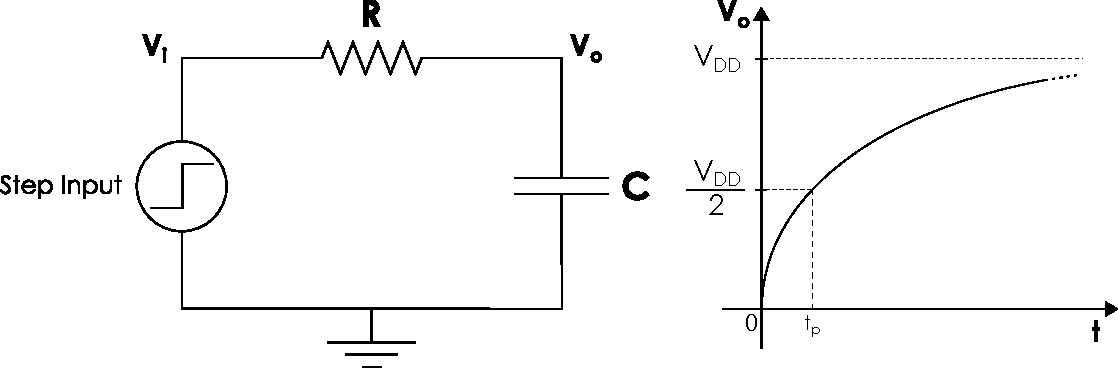
\includegraphics[width=105mm]{Figures/Background/rc_circuit.pdf}
    \caption{First order RC circuit and temporal response to step input.}
    \label{fig:rc_circuit}
\end{figure}

\begin{equation}
    V_o=V_{DD} \cdot (1-e^{t/\tau})
    \label{eq:firtst_order}
\end{equation}

Solving Equation~\ref{eq:firtst_order} for $V_o=\frac{V_{DD}}{2}$, the propagation delay is a function of the supplied voltage, of $R$ and $C$, Equation~\ref{eq:tp}.


\begin{equation}
    t_p=ln(1-\frac{V_{DD}}{2 \cdot V_{DD}})\cdot\tau=0.69\cdot\tau
    \label{eq:tp}
\end{equation}


From all the logic paths (sequence of logic gates) that connect two registers, the one which presents the largest sum of the propagation delay limits the overall maximum frequency that the \acrshort{cmos} circuit can operate, establishing itself as the critical path of the circuit, Figure~\ref{fig:critical_path}.

\begin{figure}[htb]
    \centering
    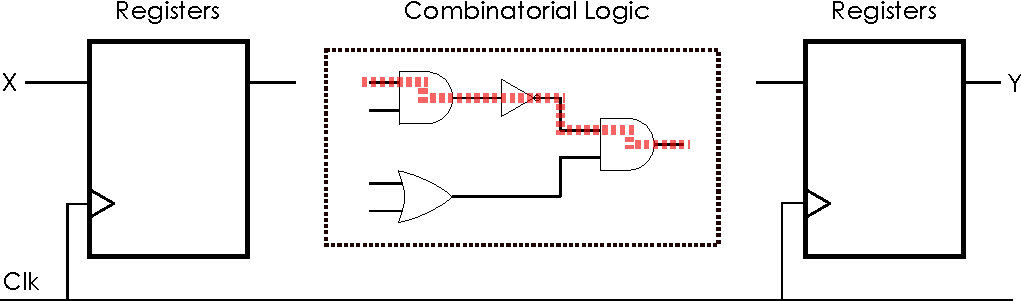
\includegraphics[width=130mm]{Figures/Background/comb_logic.pdf}
    \caption{Critical path between two registers (red dashed line).}
    \label{fig:critical_path}
\end{figure}

In this way, when scaling the circuit's operating frequency, it is only possible to increase it until it matches the inverse of the critical path propagation delay. When raising the frequency ahead of this value, the critical path is violated, meaning that when the next clock cycle starts, the output of the combinatorial logic may not be the correct one.

% When manufacturers set the digital circuit's operating frequency, they never go up to the maximum possible frequency, leaving a safe operating margin. This margin exists to guarantee correct and safe operation under process, voltage and temperature (\acrshort{pvt}) variation.



\subsection{Voltage guardband, PVT Variation and aging}

After the release of the digital circuit, silicon vendors deal with variations of their devices' specifications. On the design stage of the circuit, these variations need to be predicted and accounted for, guaranteeing the correct operation of the circuit throughout time and range of conditions that the circuit will be exposed to.

Process, voltage and temperature (\acrshort{pvt}) variation and aging impact the circuit in different manners and the solution for all is to put in place a voltage guardband, Figure~\ref{fig:voltage_guardband}. This voltage guardband increases the circuit nominal voltage from the best-case operating voltage selected from the transistors and gates' intrinsic characteristics.
In Equation~\ref{eq:tp}, the propagation delay computation is performed considering the best-case operating voltage. However, when the silicon vendor opts to put in place a voltage guardband, increasing the supplied voltage (overvoltage), the propagation delay will follow Equation~\ref{eq:tp_v_scaling}, where $V_{Threshold}$ depends on the transistors (and so, it does not depend on the supply voltage value) and $V_{Supply \: Voltage}$ is the controlled parameter. Figure~\ref{fig:voltage_scaling} illustrates the logic gate step response for over and undervoltage. Increasing the supply voltage will make the transistors switch faster, while decreasing it, reduces the switching pace.



\begin{equation}
    t_p=ln(1-\frac{V_{Threshold}}{V_{Supply \: Voltage}})\cdot\tau
    \label{eq:tp_v_scaling}
\end{equation}


\begin{figure}[!htb]
    \centering
  \begin{subfigmatrix}{2}
    \subfigure[Voltage Guardband]{
    \centering
    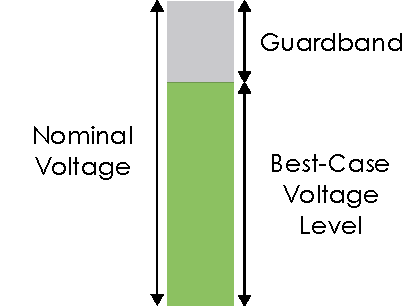
\includegraphics[height=4cm]{Figures/Background/voltage_guardband_bar.pdf}
    \label{fig:voltage_guardband}}
    \subfigure[First order circuit step response with changing supply voltage ($V_{sp}$).]{
    \centering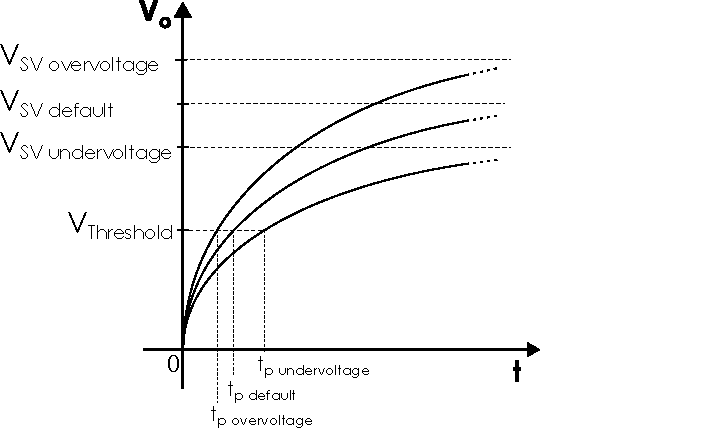
\includegraphics[height=7cm]{Figures/Background/v_scaling.pdf}
    
    \label{fig:voltage_scaling}}
  \end{subfigmatrix}
  \caption{Voltage guardband ensures reliability by making the transistors switching faster.}
\end{figure}

The work of Leng \textit{et al.}~\cite{leng_safe_2015} analyzes the voltage guardband of different applications and creates a statistical analysis procedure to predict the $V_{min}$ (the best case voltage level, Figure~\ref{fig:voltage_guardband}) depending on the collected performance counters. For the voltage guardband analysis, Leng \textit{et al.} used 57 representative programs run on four different GPUs of two different architectures. The testing procedure consists of running each program 1000 times. After which a $12mV$ undervoltage is performed on the GPU core if every run is successful, repeating the procedure until a fault occurs. The faults can be of two types: runtime error, such as segmentation fault, silent data corruption or OS crash, and incorrect output (the results of the undervolt run being different from the run with default voltage). The results of Leng's work help us infer the contribution and manifestation of each type of variation on GPUs.


\subsubsection{Process variation and aging}

Process variation and aging impact the circuit in different ways. Process variation is related to the modern fabrication process of silicon. It results from imperfections in the lithography and dopant diffusion, affecting the transistors' dimensions (for example, length and oxide thickness). This dimensionality change between the transistors can occur either intra-die, when devices from the same die present different features depending on their locations and inter-die, meaning that devices from one die can present different traits from devices from another batch of dies. The process variation affects the speed of transistors and the overall circuit characteristics by varying the device voltage threshold and speed \cite{schemmert_threshold-voltage_1974}\cite{thomas_core_2016}. Such variations are inherent to the fabrication process. Even though silicon manufacturers try to reduce this impact, such variation will always occur as a \textit{static} variation after the release of the chip to the market.

Aging of the CMOS circuits is a reflection of ongoing chip temperature variation and supply voltage change. The continuous variation of these two factors induces \textit{Bias Temperature Instability} (\acrshort{bti}) and  \textit{Hot Carrier Injection} (\acrshort{hci}). \acrshort{bti} causes threshold voltage shifts over long periods due to the presence of voltage stress at the transistors' gate. On the other side, \acrshort{hci} is caused by the acceleration of carriers (electrons/holes) under lateral electric fields in the channel of MOS devices. The acceleration can get up to the point where the carriers gain enough energy and momentum to cause damage, degrading mobilities and again, changing the threshold voltages 
\cite{sapatnekar_what_nodate}.

The occurrence of these phenomenons raises the possibility of the circuit stopping to meet its specifications. Hence, a circuit that is dimensioned without any headroom (not sufficiently large voltage guardband) may not be able to cope with the process variation - producing a not working circuit; or stopping to work overtime due to aging.

Leng \textit{et al.}~\cite{leng_safe_2015} tested the influence of process variation by running the set of benchmarks on multiple GPUs of the same model, achieving a maximum variability of 0.07V for the same benchmarks. The measured differences for process variation have a relatively low and uniform impact across all tested programs. This result indicates that this factor does not have a sufficiently high impact to be the leading root cause determining the $V_{min}$ and guardband size.


The variability of aging was not possible to measure directly. However, it is plausible to assume that this effect should produce a similar contribution to process and temperature variation \cite{leng_safe_2015}.

\subsubsection{Voltage variation}

Running the circuit at an increased voltage compared to the required at target frequency for typical workloads results in a faster circuit. This increment in performance allows for inserting an extra timing margin in each clock cycle, Figure~\ref{fig:timming_guardband}. 

\begin{figure}[!htb]
  \begin{subfigmatrix}{2}
    \subfigure[Static Margin]{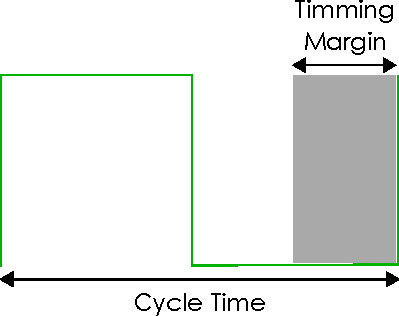
\includegraphics[height=4.5cm]{Figures/Background/static_margin.pdf}}
    \subfigure[Reduced Voltage Margin]{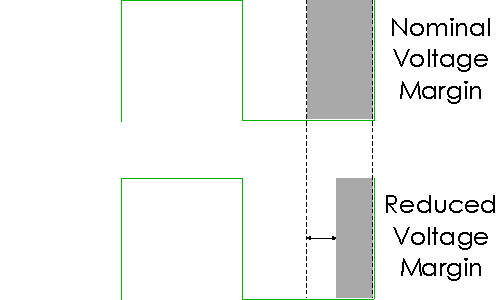
\includegraphics[height=4.5cm]{Figures/Background/reduced_voltage_margin.pdf}}
  \end{subfigmatrix}
  \caption{Voltage guardband ensures reliability by effectively inserting extra timing margin.}
  \label{fig:timming_guardband}
\end{figure}

This timing margin is of extreme importance to cope with voltage noise, the leading cause of voltage variation during the circuit execution. Voltage noise is mainly induced by $di/dt$ droop. This phenomenon makes the actual measured voltage applied to the circuit components, as formulated in Equation \ref{eq:Vactual}, depend on the rate of change of the current being drawn. 

\begin{equation}
    \label{eq:Vactual}
    V_{actual} = V_{DD}-L*\frac{di}{dt}
\end{equation}

The runtime workload intensity variation induces the $di/dt$ droop due to the rapid and significant change in current demand from the various circuit functional blocks \cite{thomas_core_2016}. Thus, in the case of processors, the workload type can directly impact voltage noise. A program that induces a bigger $di/dt$ droop will need to have a bigger voltage guardband.

\subsubsection{Temperature variation}

Temperature variation occurs both due to changing on the environmental temperature as well, due to the temperature dissipated as heat by the transistors on the circuit. The temperature affects the transistors by changing the carriers' mobility ($ \mu [\frac{cm^2}{V\cdot s}]$), and threshold voltage \cite{wolpert_temperature_2012}.

The carriers' mobility $ \mu $ describes the drift velocity of a particle in an applied electric field, thus the transistor's capability to drive electric current. MOS transistors carriers mobility presents a very complex temperature dependence; however, in general, the mobility is said to decrease with temperature increase. In the case of threshold voltage, their rate of change also follows the same principle of the carriers mobility, however having a more straightforward dependency of decreasing linearly with temperature increase.

The work of Freijado \textit{et al.}~\cite{freijedo_modeling_2012} created a model that tries to encompass all possible variations and test the impact that temperature has on the propagation delay. The designed model predicts that the propagation delay increases linearly with the temperature increase, which would imply that the size of the voltage guardband reduces with temperature rise. However, Leng \textit{et al.}~\cite{leng_safe_2015} tested the benchmarks mentioned above at two distinct temperatures (40ºC and 70ºC) while measuring the $V_{min}$. The temperature change only caused a voltage guardband size variation of $0.02V$ between the two temperatures, concluding that between these two temperatures, there is no practical effect of temperature variation. 

\subsection{Power Consumption}
\label{sec:power_consumption}
On a CMOS circuit, the total consumed power is decomposed into the dynamic and static parts, Equation \ref{eq:power}.

\begin{equation}
    P_{CMOS} = P_{dynamic} + P_{static}
    \label{eq:power}
\end{equation}

The dynamic power relates to the power consumed by the transistors flipping stages (inverting the logic values), and correspond to the power of charging and discharging the internal net capacitances. This value is proportional to the frequency that this change occurs. Equation \ref{eq:dynpower} represents the general formulation of the dynamic power, where $a$ represents the device utilization factor, $C$ the total capacitance of the circuit, $V$ the circuit supplied voltage, and $f$ the frequency of operation \cite{gonzalez_supply_1997}.

\begin{equation}
    P_{dynamic} = aCV^2f
    \label{eq:dynpower}
\end{equation}

On the other hand, the static part of the power consumption comprehends three components: $P_{leakage}$, $P_{short-circuit}$ and $P_{DC}$ \cite{mei_survey_2016}. The leakage power is independent of the transistors flip, and it represents the flow of electrons between the transistors' source, drain, and gate, known as leakage current. The short-circuit power comes from the instantaneous short-circuit connection between the supply voltage and the ground when the transistor flips. Finally, the Direct Current (DC) power corresponds to the power needed for powering the circuit. Equation \ref{eq:cmosstatic} represents the total power consumption sources.

\begin{equation}
    P_{static} = P_{leakage} + P_{short-circuit} + P_{DC}
    \label{eq:cmosstatic}
\end{equation}

Usually, the dynamic power dominates the total power consumption of a circuit. However, with the current reduction of the transistors manufacturing size, the static power is becoming more of a significant part \cite{s._hong_modeling_2012} \cite{hong_integrated_2010}. Nevertheless, as a common reference, and due to the usually higher weight of the dynamic power on the total power consumption, the power used by a CMOS circuit usually changes linearly with the clock frequency and quadratically with the supplied voltage.


%%%%%%%%%%%%%%%%%%%%%%%%%%%%%%%%%%%%%%%%%%%%%%%%%%%%%%%%%%%%%%%%%%%%%%%%
\section{Dynamic Voltage and Frequency Scaling}
\label{section:DVFS}

The widespread use of GPUs in both supercomputers and personal computing machines comes at the cost of a significant increase in power consumption. While a typical modern CPU consumes about 50 to 100W, it is common to see GPUs consuming between 200 and 300W of power. With these figures, the use of energy efficiency techniques to try to reduce power consumption becomes a vital issue.

As stated in Section~\ref{sec:power_consumption}, the power consumption of a CMOS circuit increases linearly with the operating frequency and quadratically with the supplied voltage. Thus, a direct manner of reducing this figure is by directly acting on these two parameters. 
Dynamic Voltage and Frequency Scaling (\acrshort{dvfs}) is a power management technique which performs "on the fly" control of frequency and voltage. \acrshort{dvfs} allows for an energy efficiency improvement by matching the GPU utilization to voltage and frequency settings. When the GPU is idle, the frequency is lowered, and when it is active, the frequency is increased. As presented in the previous section, the frequency scaling also implies a change in voltage to accommodate the critical path timing constraints' fulfillment. 

In general, the applied voltage level $V$ is a function of the current operating frequency $f$, in the form of $V(f)$. Therefore, by intelligently controlling the clock frequency, the required voltage level for stable operation of the circuit can also be reduced, leading to further power savings.

In general, modern GPU boards have independent control over two pairs of frequency and voltage. Each pair (or domain) acts on a distinct part of the GPU, intending to maximize the performance or reduce the power consumption. The first domain concerns the GPU core, acting on all \acrshort{sm}/\acrshort{cu}s, the cache, and the interconnection fabric. The second affects the \acrshort{dram} chips that compose the video memory. 

The clock frequency is an independently controlled variable, and its change directly reflects on the performed achieved by the GPU. An increase in the clock frequency of the core results in an improvement of the \acrshort{sm}/\acrshort{cu} execution speed, while the same change in the memory frequency will increase the \acrshort{dram} I/O throughput \cite{mei_survey_2016}. The voltage level of each domain is dependent on the clock frequency being computed based on tests performed by the manufacturer to ensure the correct operation of the circuit, independently of the workload.

The two major GPU silicon vendors, AMD and NVIDIA, have on their products the concept of performance levels. A performance level is a pair of frequency and voltage that can be applied to the \acrshort{gpu} \acrshort{dvfs} domains. These vary from low power and performance levels to high performance and high power ones. The idea of having multiple performance levels is to be able to always be at the best point of operation.  In the case of the GPU that is going to be used in the experimental phase of the dissertation, the GPU core has eight performance levels, while the memory has only four. Table \ref{tab:gpulevels} shows the reference values for frequency and voltage for each of the core and memory performance levels. The frequency and voltage of increasing performance levels reflect the expected behavior, increasing the voltage to accommodate the frequency boost.


\subsection{Control Mechanism}
\subsection{GPU DVFS Characterization}


\subsection{DVFS Optimization}
\label{section:DVFS_opt}

\subsubsection{Coupled V-F - Conventional DVFS optimization}

frequency scaling with tied voltage scaling

\subsubsection{Decoupled V-F - Non-conventional DVFS optimization}

decoupled frequency and voltage scaling

%%%%%%%%%%%%%%%%%%%%%%%%%%%%%%%%%%%%%%%%%%%%%%%%%%%%%%%%%%%%%%%%%%%%%%%%
\section{Undervoltage behaviour and imprecision tolerant applications}
\label{section:und_beh}